% !TeX spellcheck = it_IT
% !TEX TS-program = pdflatex
% !TEX root = ../main.tex


% ********************************************************************
\section{Prototipo}
\label{sec:prototipo}
% ********************************************************************


\subsection{Login e autenticazione}




\subsection{Dashboard donatore}
La \textit{dashboard} del donatore è l'interfaccia attraverso la quale i donatori possono interagire direttamente con la piattaforma a seguito della procedura di autenticazione. Essa è progettata per fornire una visione sinottica e intuitiva delle iniziative di \gls{cf} attive, permettendo all'utente di monitorare variabili critiche relative al loro stato di avanzamento, come \textit{budget} raggiunto e scadenza. \\
Una volta selezionata l’iniziativa di interesse, l’utente ha la possibilità di procedere con l’operazione di donazione. Il sistema adotta il modello di raccolta \textit{keep-it-all}, in base al quale l’Ente beneficiario conserva i fondi raccolti anche nel caso in cui l’obiettivo economico prefissato non venga raggiunto entro i termini stabiliti. \\
Tale scelta progettuale risulta coerente con la tipologia degli Enti autorizzati alla creazione delle iniziative, individuati esclusivamente in Enti del Terzo Settore e \gls{onp}, per i quali anche contributi parziali possono risultare funzionali al perseguimento delle finalità sociali.


\begin{figure}[!b]
	\centering
	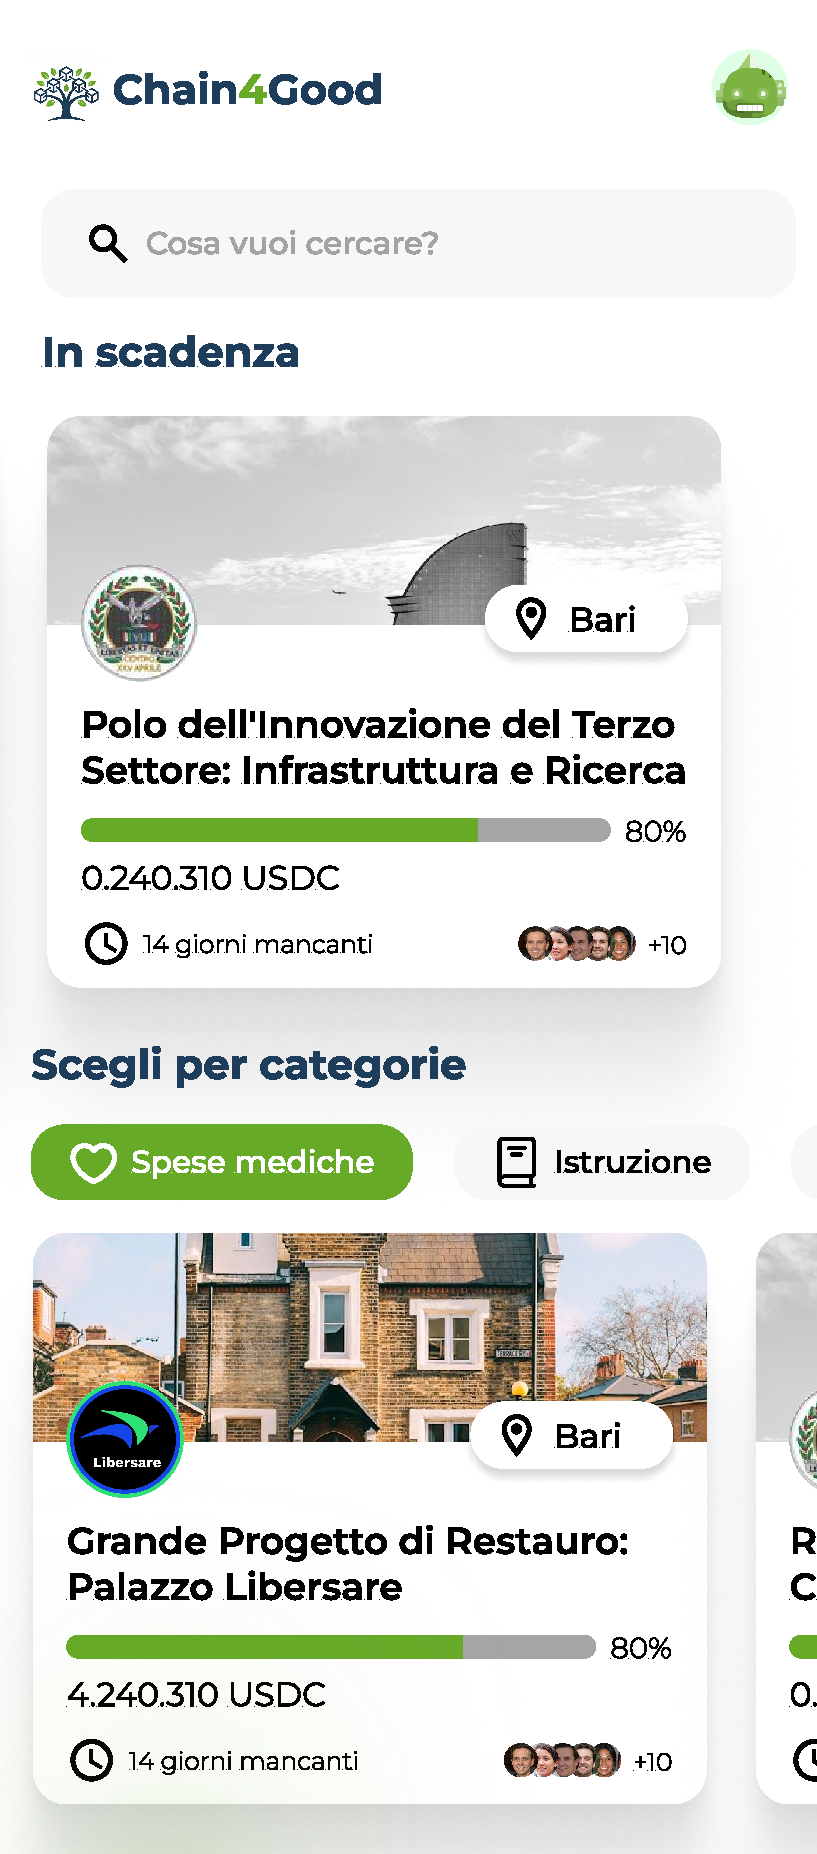
\includegraphics[width=0.45\textwidth]{images/Home.pdf}
	\caption{Dashboard del donatore}
	\label{fig:dashboard-donatore}
\end{figure}

\subsection{Creazione progetto}
La creazione di un progetto costituisce l’atto attraverso il quale il beneficiario formalizza la propria proposta sulla piattaforma. Si tratta di una procedura articolata in due step (\ref{fig:inserimento progetto}):

\begin{itemize}
	\item durante il primo step, il beneficiario deve specificare il nome del progetto, la categoria (come istruzione, ambiente), l’obiettivo economico e il termine temporale della raccolta. Queste variabili sono essenziali per automatizzare la gestione dei fondi in modalità \textit{trustless}, in quanto lo \textit{Smart Contract} li utilizza per determinare il successo della campagna;
	
	\item durante il secondo step, invece, il sistema impone l'inserimento di un piano dettagliato delle spese. Tale prospetto non ha solo finalità informative, in quanto mira ad incrementare la credibilità dell'iniziativa e a consolidare il rapporto fiduciario con i donatori. Inoltre, queste informazioni fungono da parametro di confronto per i sostenitori, ai quali spetta il compito di valutare la coerenza degli obiettivi dichiarati con le motivazioni relative alle richieste di spesa.
	
\end{itemize}


\begin{figure}[!h]
	\centering
	\begin{minipage}{0.45\textwidth}
		\centering
		\includegraphics[width=\textwidth]{images/nuovo_progetto1.pdf}
	\end{minipage}
	\hspace{0.9cm}
	\begin{minipage}{0.45\textwidth}
		\centering
		\includegraphics[width=\textwidth]{images/NuovoProgetto 2.pdf}
	\end{minipage}
	\caption{Inserimento di un nuovo progetto}
	\label{fig:inserimento progetto}
\end{figure}



\subsection{Inserimento e valutazione spesa}

A differenza dei sistemi centralizzati in cui l'Ente ha piena e immediata disponibilità del \textit{budget} donato, l’architettura proposta prevede che i fondi raccolti rimangano vincolati all'interno di uno \textit{Smart Contract}. \\
Per accedere a tali risorse, il beneficiario deve formalizzare una "Richiesta di Spesa" (\ref{fig:valutazione-spesa}) attraverso l'inserimento dei seguenti parametri: identificativo della spesa, importo richiesto, finalità dell'esborso e preventivo. \\
Una volta sottomessa la richiesta, la piattaforma permette ai donatori di analizzare la documentazione ed esercitare il proprio diritto di voto.

\begin{figure} [h]
	\centering
	\begin{minipage}{0.45\textwidth}
		\centering
		\includegraphics[width=\textwidth]{images/nuova_spesa.pdf}
	\end{minipage}
	\hspace{0.9cm}
	\begin{minipage}{0.45\textwidth}
		\centering
		\includegraphics[width=\textwidth]{images/valutazione_spesa.pdf}
	\end{minipage}
	\caption{Valutazione di una richiesta di spesa}
	\label{fig:valutazione-spesa}
\end{figure}



\subsubsection{Meccanismo di validazione}
Per garantire l'operatività del sistema ed evitare lo stallo decisionale, lo \textit{Smart Contract} è stato programmato per agire secondo le seguenti regole:
\begin{itemize}
	\item La richiesta è approvata se la maggioranza dei votanti (rappresentata dalla comunità di individui che finanzia un'iniziativa) esprime un parere favorevole. In presenza di una partecipazione parziale, la soglia di maggioranza viene ricalcolata in funzione dei soli voti espressi.
	\item Qualora non venga registrata alcuna attività di voto, il sistema approva automaticamente la richiesta.
\end{itemize}

Al soddisfacimento dei requisiti di approvazione, lo \textit{Smart Contract} esegue in modo autonomo e irreversibile il trasferimento della somma raccolta verso il \textit{Wallet} del beneficiario.

